\chapter{Fenómenos Ondulatorios}% \label{lbl-fenomenos}
% Refelexion
\section{Reflexión}% \label{lbl-reflexion}
\subsection{Definición}
Es el cambio de dirección que experimenta un onda cuando choca contra una superficie y regresa al medio del cual provenie. Las superficies planas y duras reflejan más. Esto ocurre con diversas ondas como luz, sonido y las ondas en la superficie del agua.

\begin{figure}[H]
  \centering
  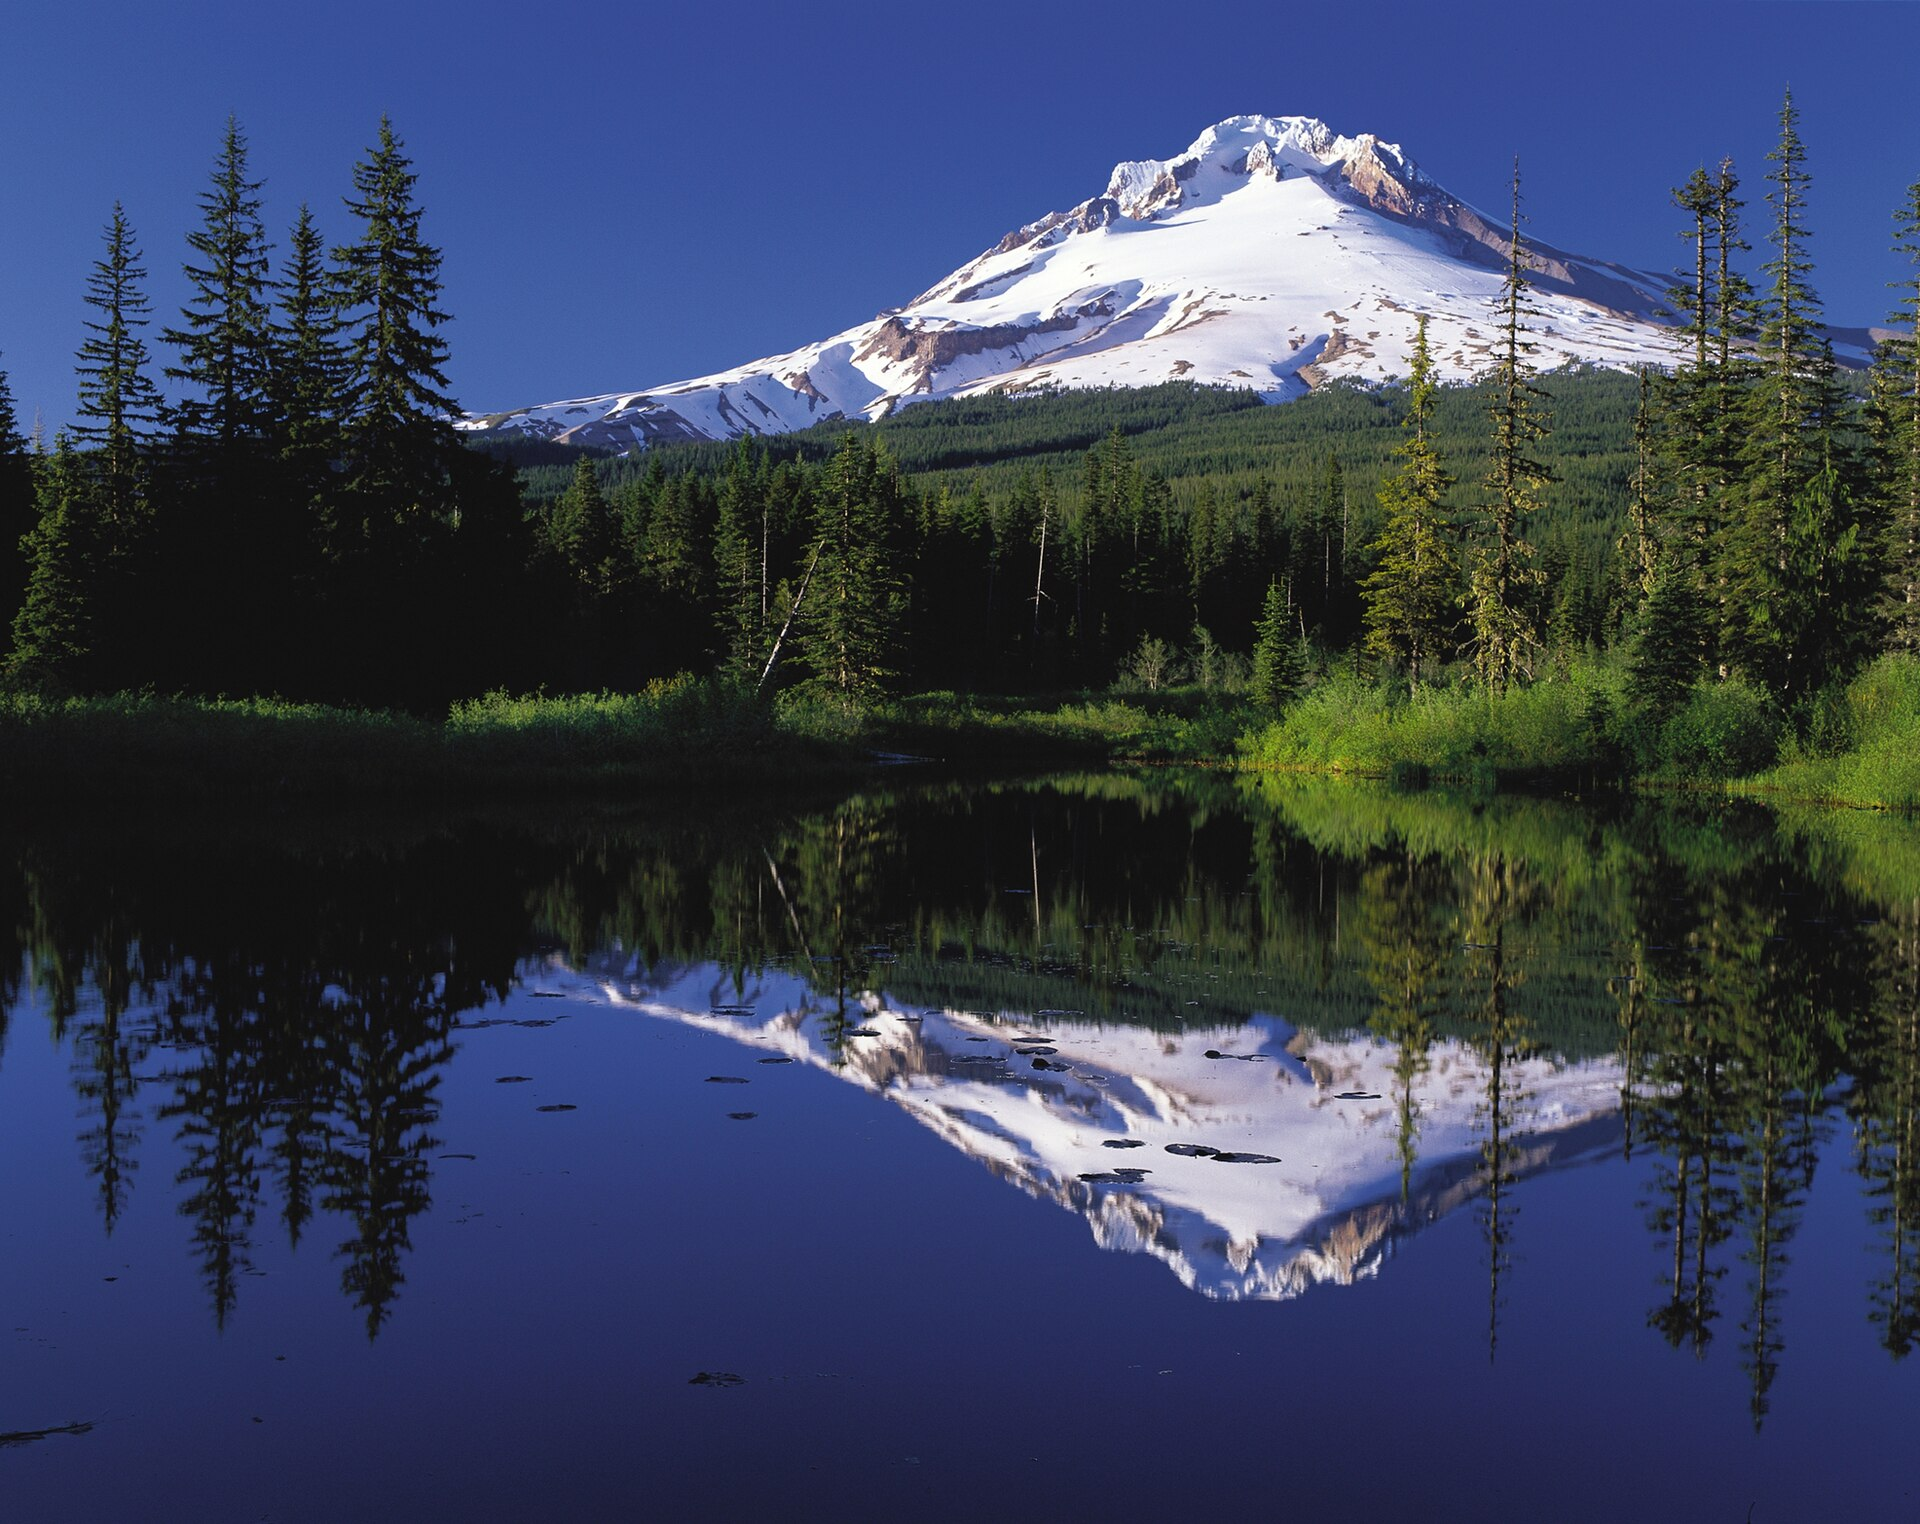
\includegraphics[scale=0.15]{imagenes/reflexion_monte.png}
  \caption{Reflexión en el agua\cite{wikireflexion}}
\end{figure}

El \textbf{eco} es un ejemplo de este fenómeno. Cuando una onda sonora choca contra una superficie, parte de la energía de la onda se refleja. Esto se percibe como un sonido distinto al original, debido a la separación temporal entre la onda emitida y reflejada. También se puede mencionar la \textbf{reverberación}, en este caso en un reflejo continuo de la onda de sonido.

La luz es otro caso preponderante. Toda la luz percibida por el ojo humano es el resultado de un rebote de las ondas de luz al chocar con multitud de superficies. Cuando el ojo no recibe ondas de luz, como en lugares oscuros o en la noche, entonces percibe oscuridad. La luz de estrellas lejanas llega constantemente hasta el planeta tierra, aunque durante el día es opacada por la luz solar emitida por el sol ubicado en el centro del sistema solar donde se encuentra la tierra.

\subsection{Tipos}
\input{fenomenos/reflexion/tipos.tex}
% Refraccion
\section{Refracción}
\subsection{Definición}
Cambio de dirección que experimenta una onda al pasar de un medio a otro con diferenta velocidad de propagación. Esto ocurre porque la onda cambia de velocidad al entrar en el nuevo medio, lo que provoca que se desvíe de su trayectoria original.

Cada medio, debido a sus propiedades físicas, tiene una velocidad de propagación diferente. Cuando las ondas interactuan con cada medio, su trayectoria está condicionada por la velocidad con la que se mueve dentro de se medio\cite{sncrfrlight}.

\begin{figure}
  \centering
  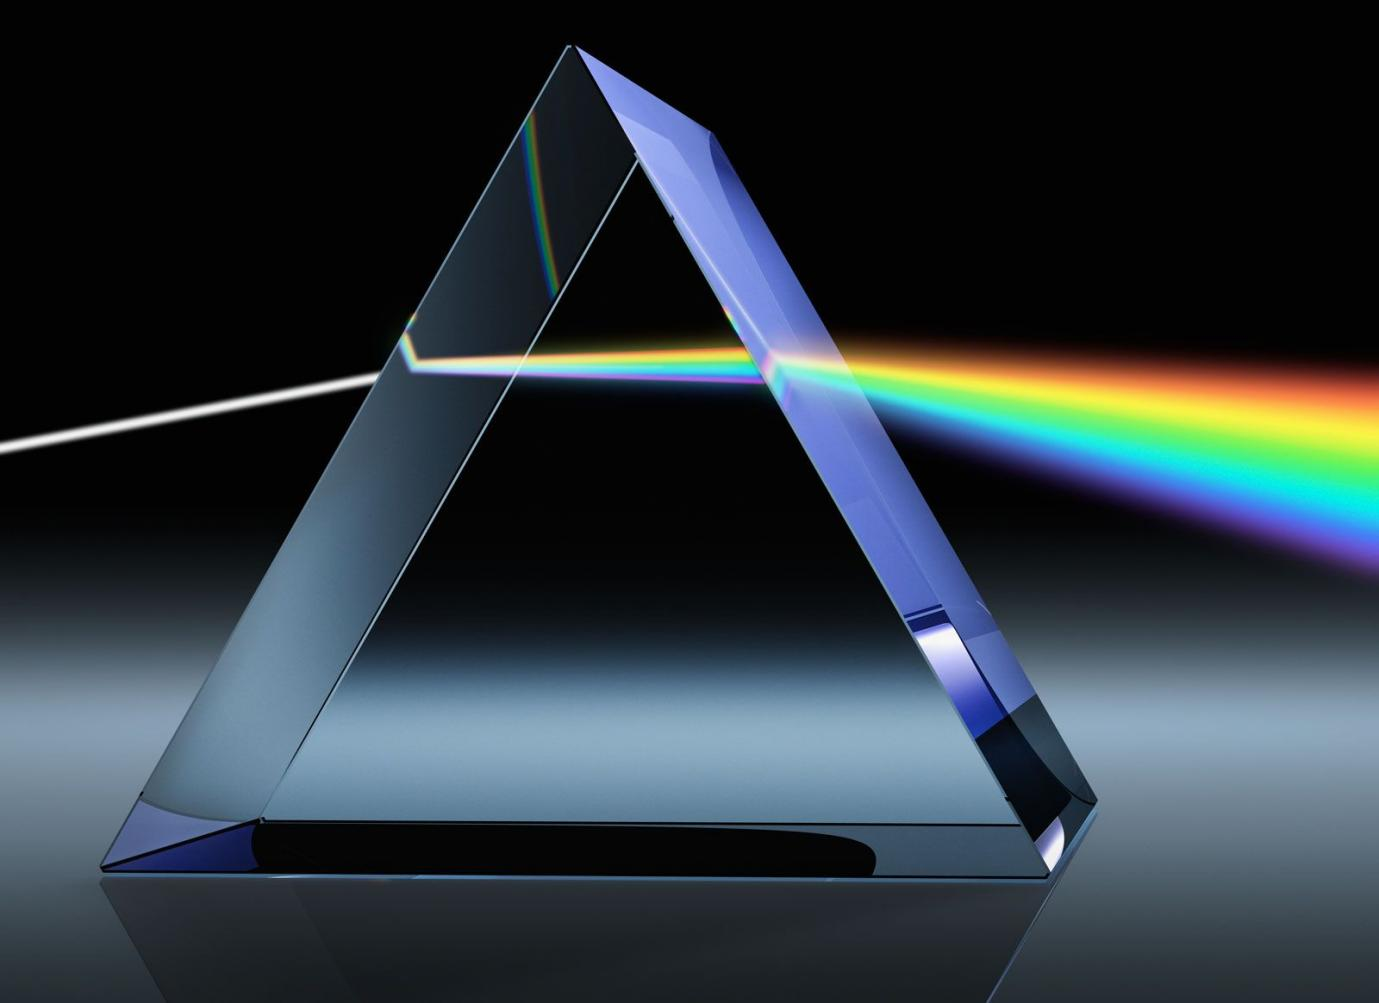
\includegraphics[scale=0.5]{imagenes/prisma.png}
  \caption{Refracción en un prisma\cite{cstmglassprism}}
\end{figure}

La refracción ocurre todo el tiempo. Se usa para enfocar la luz y crear imagenes claras mediante lentes de gafas, cámaras telescopios, microscopios y otros. Los arcoiris ocurren cuando la luz se refracta en las gotas de lluvia. Los objetos en el agua parecen estar doblados por efecto de la refracción.

Un gran ejemplos son los prismas hechos cristal o vidrio. La luz blanca, que es la combinación de todos los colores, al pasar a través del prisma se descompone en un espectro de colores como un arcoiris. Esto se debe a la distinta longitud de onda de los colores en el rango de luz visible.

\subsection{Descripción Matemática}
\input{fenomenos/refraccion/matematica.tex}
% Difraccion
\section{Difracción}
\subsection{Definición}
Ocurre cuando una onda se encuentra con un obstáculo o abertura y se desvía, propagándose en diferentes direcciones. Puede producirse de distinas formas dependiendo del tamaño del obstáculo y la longitud de onda de la onda. Puede ocurrir alrededor o a través de un obstáculo o abertura. En este proceso se crean zonas en donde las onda no llegan o se cancelan mediante interfernecia \textbf{destructiva}.

\begin{figure}[H]
  \centering
  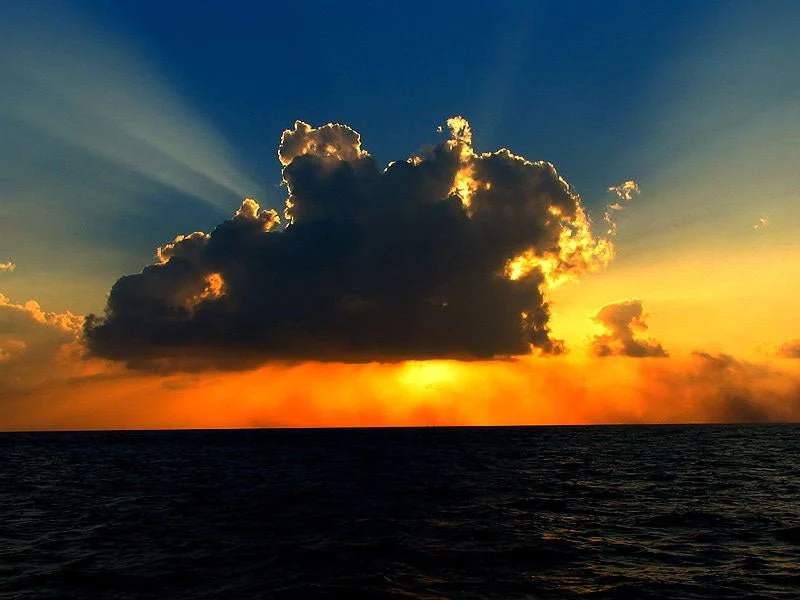
\includegraphics[scale=0.3]{imagenes/difraccion_nube.png}
  \caption{Difracción en las nubes\cite{rnbsymdfr}}
\end{figure}

Una forma simple de ver la difracción de ondas es colocar los dedos de una mano en frente de una fuente de luz y cerrarlos lentamente observando la luz pasar a través de ellos. A medida que los dedos se acercan unos a otros la luz forma patrones de lineas entre los dedos. Otra situación de esto es la luz difractada por las nubes. Esas lineas son patrones de difracción\cite{sncdfrlight}.

\subsection{Tipos}
\input{fenomenos/difraccion/tipos.tex}
% Absorcion
\section{Absorción}
\subsection{Definición}
Proceso por el cual un medio absorbe energía de una onda que lo atraviesa, reduciendo su amplitud y eventualmente su intensidad. Ocurre cuando la energía de la onda se transforma en otra forma de energía, generalmente calor, dentro del material.

Esto se puede observar en el espectro de absorción de los hojas. La clorofila no absorbe toda la luz solar uniformemente. Las moléulas de clorofila preferentemente absorben la luz roja (con picos de aborción de $600-700 nm$ del \EspectroElectromagnetico) y azul (con picos de aborción de $400-500 nm$) para usar en la fotosíntesis, pero mucho menos en la luz verde (picos de absorción de $500-600 nm$) es absorbida y por tanto una gran cantidad es reflejada\cite{doncontrolhojas}.

\begin{figure}[H]
  \centering
  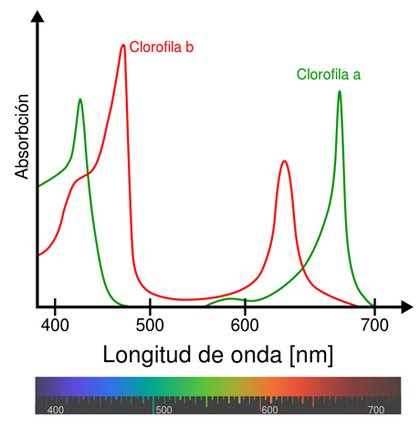
\includegraphics[scale=0.6]{imagenes/absorcion_hojas.png}
  \caption{Espectro de absorción de las hojas\cite{doncontrolhojas}}
\end{figure}

